\documentclass[10pt]{book}

%These tell TeX which packages to use.
\usepackage{array,epsfig}
\usepackage{amsmath}
\usepackage{amsfonts}
\usepackage{amssymb}
\usepackage{amsxtra}
\usepackage{amsthm}
\usepackage{mathrsfs}
\usepackage{color}
\usepackage{enumitem}
%\usepackage{mdframed}
\usepackage[most]{tcolorbox}
\usepackage{pgfplots}
\pgfplotsset{compat=1.6}

\pgfplotsset{soldot/.style={color=black,only marks,mark=*}} \pgfplotsset{holdot/.style={color=black,fill=white,only marks,mark=*}}

%Here I define some theorem styles and shortcut commands for symbols I use often
\theoremstyle{definition}
\newtheorem{defn}{Definition}
\newtheorem{thm}{Theorem}
\newtheorem{cor}{Corollary}
\newtheorem*{rmk}{Remark}
\newtheorem{lem}{Lemma}
\newtheorem*{joke}{Joke}
\newtheorem{ex}{Example}
\newtheorem*{soln}{Solution}
\newtheorem{prop}{Proposition}

\newcommand{\lra}{\longrightarrow}
\newcommand{\ra}{\rightarrow}
\newcommand{\surj}{\twoheadrightarrow}
\newcommand{\graph}{\mathrm{graph}}
\newcommand{\bb}[1]{\mathbb{#1}}
\newcommand{\Z}{\bb{Z}}
\newcommand{\Q}{\bb{Q}}
\newcommand{\R}{\bb{R}}
\newcommand{\C}{\bb{C}}
\newcommand{\N}{\bb{N}}
\newcommand{\M}{\mathbf{M}}
\newcommand{\m}{\mathbf{m}}
\newcommand{\MM}{\mathscr{M}}
\newcommand{\HH}{\mathscr{H}}
\newcommand{\Om}{\Omega}
\newcommand{\Ho}{\in\HH(\Om)}
\newcommand{\bd}{\partial}
\newcommand{\del}{\partial}
\newcommand{\bardel}{\overline\partial}
\newcommand{\textdf}[1]{\textbf{\textsf{#1}}\index{#1}}
\newcommand{\img}{\mathrm{img}}
\newcommand{\ip}[2]{\left\langle{#1},{#2}\right\rangle}
\newcommand{\inter}[1]{\mathrm{int}{#1}}
\newcommand{\exter}[1]{\mathrm{ext}{#1}}
\newcommand{\cl}[1]{\mathrm{cl}{#1}}
\newcommand{\ds}{\displaystyle}
\newcommand{\vol}{\mathrm{vol}}
\newcommand{\cnt}{\mathrm{ct}}
\newcommand{\osc}{\mathrm{osc}}
\newcommand{\LL}{\mathbf{L}}
\newcommand{\UU}{\mathbf{U}}
\newcommand{\support}{\mathrm{support}}
\newcommand{\AND}{\;\wedge\;}
\newcommand{\OR}{\;\vee\;}
\newcommand{\Oset}{\varnothing}
\newcommand{\st}{\ni}
\newcommand{\wh}{\widehat}
%Pagination stuff.
\setlength{\topmargin}{-0.75in}
\setlength{\oddsidemargin}{0in}
\setlength{\evensidemargin}{0in}
\setlength{\textheight}{9.in}
\setlength{\textwidth}{6.5in}
\pagestyle{empty}
\begin{document}
\begin{flushleft}
Name:\underline{\hspace{13cm}}Date:\underline{\hspace{2cm}}
\end{flushleft}
\begin{center}
{\Large Math 1041-012 \hspace{0.5cm} Section 2.7: Derivatives and Rates of Change}
\end{center}
%\vspace{0.2 cm}
\begin{tcolorbox}
\subsection*{Recall the basic problems}
\begin{itemize}
    \item Find the equation of the tangent line to a curve.
    \item Find the \textit{instantaneous rate of change}.
\end{itemize}
\end{tcolorbox}
\begin{figure}[h!]
    \centering
    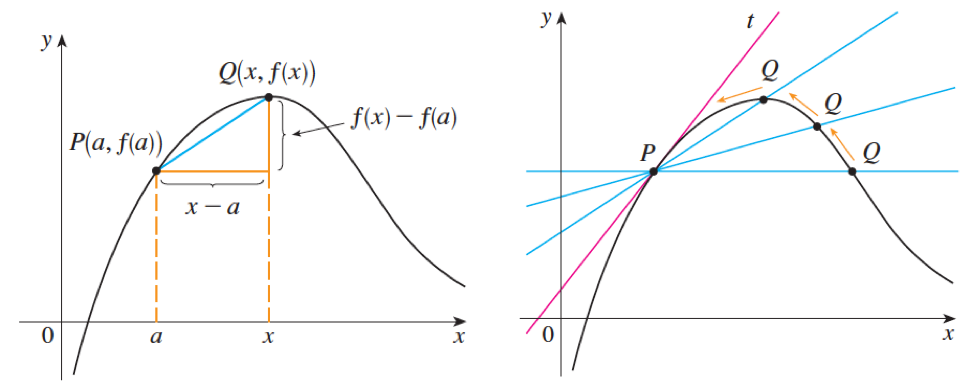
\includegraphics[scale=0.7]{fig1.png}
\end{figure}
\begin{tcolorbox}
\subsection*{Definition} The \textbf{tangent line} to the curve $y=f(x)$ at the point $P(a,f(a))$ is the line through $P$ with slope
\begin{itemize}
    \item[(1)] $\displaystyle
m=\lim_{x\rightarrow a}\frac{f(x)-f(a)}{x-a}
$\vspace{0.5cm}
\item[(2)]$m=\displaystyle\lim_{h\rightarrow 0}\frac{f(a+h)-f(a)}{h}$
\end{itemize}
This is also called the \textit{slope of the curve} at $a$.
\end{tcolorbox}
\subsection*{Example 1: Find the equation of the tangent line}
\begin{itemize}
    \item[(a)] Find an equation of the tangent line to the parabola $y=x^2$ at the point $P(1,1)$\vspace{5cm}
    \item[(b)] Find an equation of the tangent line to the hyperbola $y=3/x$ at the point $P(3,1)$.
\end{itemize}
\raggedbottom
\clearpage
\begin{tcolorbox}
\subsection*{Velocity and Instantaneous Rate of Change}
Recall that 
\[
v_{ave}=\frac{f(t_2)-f(t_1)}{t_2-t_1}=
\]
If we let the time difference ($h=t_2-t_1$) go to zero then we get \textbf{instantaneous} velocity
\[
v(a)=\lim_{h\rightarrow 0}\frac{f(a+h)-f(a)}{h}=\textrm{slope of tangent line at $a$.}
\]
This is also the instantaneous rate of change of $y=f(x)$ with respect to $x$ when $x=a$.
\end{tcolorbox}
\subsection*{Example 2: Falling Ball}
Suppose that a ball is dropped from the upper observation deck of the CN Tower, 450 meters above the ground with position given by $s=f(t)=4.9t^2$.
\begin{itemize}
    \item What is the velocity of the ball after 5 seconds?
    \item How fast is the ball traveling when it hits the ground?
\end{itemize}
\vspace{8cm}
\begin{tcolorbox}
\subsection*{Definition of Derivative at a number}
The \textbf{derivative of a function $f$ at a number $a$} is denoted by
\[
f'(a)=\lim_{h\rightarrow 0}\frac{f(a+h)-f(a)}{h}
\]
if the limit exists. Equivalently
\[
f'(a)=\lim_{x\rightarrow a}\frac{f(x)-f(a)}{x-a}.
\]
This definition is similar to the previous ones, except we are finding a \textit{formula} $f'(a)$ in-terms of $a$. This formula will tell us the derivative of $f$ at any particular number $a$. 
\end{tcolorbox}
\raggedbottom
\clearpage
\subsection*{Example 3}
\begin{itemize}
    \item[(a)] Find the derivative of the function $f(x)=x^2-8x+9$ at the number $a$.
    \item[(b)] Use part (a) to find the slope of the curve at $x=3$.
    \item[(c)] Find an equation of the tangent line to the curve $y=f(x)$ at the point $(3,-6)$.
\end{itemize}
\vspace{8cm}
\subsection*{Example 4}
The limit below represents the derivative of some function $f(x)$ at some number $a$. State the function $f$ and the value $a$.
\[
\lim_{h\rightarrow 0}\frac{\sqrt{9+h}-3}{h}
\]
\end{document}